\tikzstyle{node}=[circle,inner sep=0.5mm,minimum size=5.25mm,draw = black]
\tikzstyle{bright}=[fill=black!14]
\tikzstyle{dark}=[fill=black!28]
\tikzstyle{lightEdgeStyle}=[black!20]

\newcommand{\numberOfNodes}{5} % must be >= 4

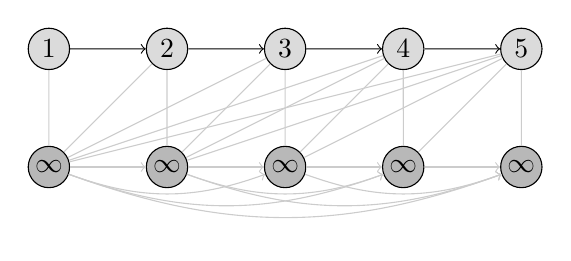
\begin{tikzpicture}[scale=1.5, bend angle = 20]

% Obere Reihe
\node(Top1) at (1,1) [node, bright] {1};
\foreach \i [evaluate = \i as \lastNode using \i-1] in {2,3,...,\numberOfNodes}
{
  \node (Top\i) at (\i,1) [node, bright] {\i}
    edge[<-] (Top\lastNode);
}

% Untere Reihe
\node(Bot1) at (1,0) [node, dark] {$\infty$};
\foreach \i [evaluate = \i as \lastNode using \i-1] in {2,3,...,\numberOfNodes}
{
  \node (Bot\i) at (\i,0) [node, dark] {$\infty$}
    edge[<-, lightEdgeStyle] (Bot\lastNode);
}

% Kanten zwischen den Reihen
\foreach \i in {1,2,...,\numberOfNodes}
{
  \foreach \j in {\i,...,\numberOfNodes}
   {
     \draw[lightEdgeStyle] (Bot\i) -- (Top\j);
   }
}

% Pfeile nach rechts
\pgfmathparse{\numberOfNodes - 2}
\foreach \i [evaluate = \i as \nextNode using \i+2] in {1,2,...,\pgfmathresult}
{
 \foreach \j [count=\nodeIndex from \nextNode] in {\nextNode,...,\numberOfNodes}
 {
   \draw[->, lightEdgeStyle] (Bot\i) to [bend right] (Bot\nodeIndex);
 }
}

\end{tikzpicture} 
